
%%% outline
%-------------------------------------------------------------------------
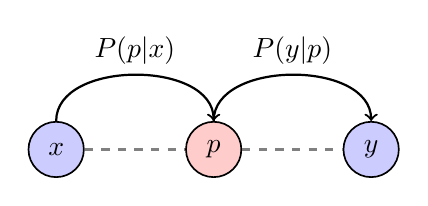
\begin{tikzpicture}

\node[draw,circle,inner sep=2pt,minimum size=2em,fill=blue!20,line width=0.6pt] (x) at (0,0) {$\seq{x}$};

\node[draw,circle,inner sep=2pt,minimum size=2em,fill=red!20,line width=0.6pt] (p) at (2,0) {$\seq{p}$};

\node[draw,circle,inner sep=2pt,minimum size=2em,fill=blue!20,line width=0.6pt] (y) at (4,0) {$\seq{y}$};

\draw[-,dashed,thick,black!50] (x.0) -- (p.180);
\draw[-,dashed,thick,black!50] (p.0) -- (y.180);
\draw[->,out=90,in=90,thick] (x.90) to node[above]{$\funp{P}(\seq{p}|\seq{x})$}(p.90);
\draw[->,out=90,in=90,thick] (p.90) to node[above]{$\funp{P}(\seq{y}|\seq{p})$}(y.90);

\end{tikzpicture}




